\subsection*{3.1 System model}
- introduce all entities in system
\noindent SCtickets introduces the following parties:
\\
\textbf{Owner}:is creator of some smart contracts which can be called by User after SCtickets verification
firstly. Normally, Owner should hold the possession of a number of smart contracts while one smart contract is only belong to one Owner.
\\
\textbf{Access Authentication Account(AAA)}:is an entity that offers SCtickets-related services including policy and verification key-pair management. Also, AAA is able to generate SCtickets and grant authorization information to User by validating all the policies corresponding to the Owner which User is intend to call. SCtickets contain mutiple arguments and provide User with ample calling message, e.g., which function in Owner can be called and valid calling timestamp period.
\\
\textbf{User}:can be treated as any application which has authority to get access to smart contracts only after obtaining valid SCtickets granted by AAA.


\subsection*{3.2 SCtickets overview}
- introduce motivation of tickets
- introduce tickets details, including type, functionality, high-level overview.
\noindent A high level description is presented in \autoref{fig:overview}.
\begin{figure}[h!]
  \centering
  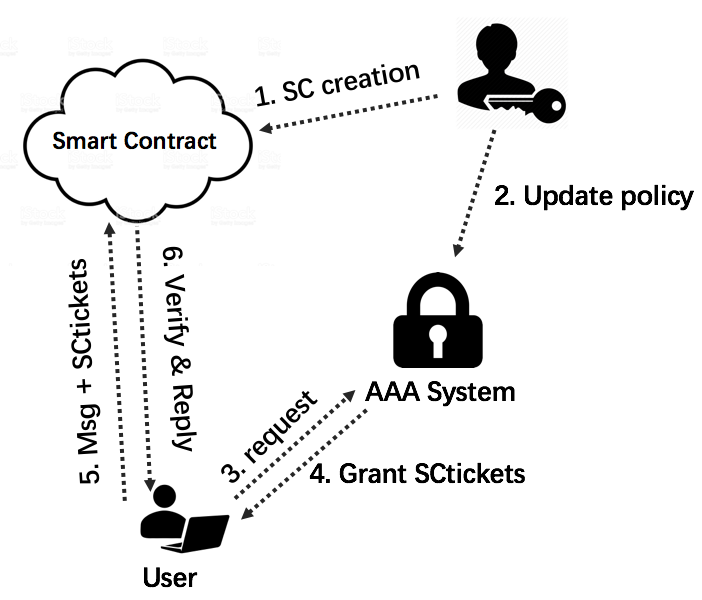
\includegraphics[width=0.7\linewidth]{fig/overview}
  \caption{A high-level overview of the SCtickets.}
  \label{fig:overview}
\end{figure}
\\\indent The central point of our design is a AAA platform that implements main functionalities: the SCtickets-related services and access policies management. The SCtickets-related services grant Users to SCtickets generated by the calling message of User and provide Owner with verification functionality corresponding to the SCtickets, while the latter functionality is used mainly for managing general access policies (e.g., insert, remove, update). Meanwhile, AAA is responsible for keeping public key and private key pair in local storage. The above-mentioned key pair is used for tickets signature and verification prcess and generated through web3.js by leveraging secp256k1 elliptic curve, aiming not to leaking the privacy of Owner account in Ethereum.
Assume that the Owner do have a valid location(address) of its smart contract in Ethereum network, every calling though different smart contracts is able to trigger a new transaction regardless of its gaslimit, gasprice.\\\indent 1 - In the first step, Owner synchronized its own policy to AAA when a new smart contract created by itself. Besides, Owner also generates new verification key-pair which is sent to AAA. AAA stores general policies corresponding to Owner’s rule as well as key pair.
\\ \indent 2 - User requests the SCtickets-generate service by sending transaction information that contains transaction message information before access to the Owner, such as msg.sender represents calling address and msg.sig represents calling specific function in Owner’s code, respectively.
\\\indent3 - The AAA notices the request and trigger SCtickets-generate service itself. First of all, AAA analyzes the parameters sent by User and determines access permission according to the policies matching. Then, if User have permission to Owner, AAA is able to generate a signature according to the SCtickets type using elliptic curve signature algorithm in Ethereum, where signer is Owner associated with its verification private key while message-to-be-signed suffix with current timestamp are based on diffrent SCtickets types accordingly. Finally, AAA transfers SCtickets to User. Tickets can be treated as a permission for Owner, like a visa for entry countries. However, if User fails to pass all the compulsory policies, AAA have right to refuse User’s access.
\\\indent4 - User send request to Owner after it hold a SCtickets. Once noticed the request, Owner firstly should verify the validation of SCtickets so as to be aware of tickets type, which smart contract is calling and executing its own code, which function can be called and the allowed calling time. Verification process is supposed to be done within Owner's code, parsing the signature to the public key corresponding to private key during signing process. Additionally, there are two types of function call, namely, external call and internal call. The former type raises a new transaction process from step 1 to step 4 repeatedly as every variable value of the SCtickets will be change in Solidity language and a new SCtickets will be granted for new User accordingly. On the other hand, the latter type just read/write internal methods without passing any SCtickets.
\\\indent5 - Every access period need to abide by blockchain timestamp in Ethereum network, leveraging UNIX global timestamp.  User can access to Owner by the expiry timestamp and, also, is able to apply for a new SCtickets in case of passing the requirements.
\\\indent6 - AAA, a strong proxy for authorizing permission and validating access, should not be a smart contract so as to every smart contract mined in blockchain is permanent and forever state and disallowed to changed while policies within AAA updates dynamically.
\\\indent7 - Owner maintains the right to refuse any calls if happens to unmatched verification despite User has been obtained valid SCtickets for the fact that malicious attack and fake signature issue.